\newif\ifshowsolutions
\showsolutionstrue
\documentclass{article}
\usepackage{listings}
\usepackage{amsmath}
%\usepackage{subfigure}
\usepackage{subfig}
\usepackage{amsthm}
\usepackage{amsmath}
\usepackage{amssymb}
\usepackage{graphicx}
\usepackage{mdwlist}
\usepackage[colorlinks=true]{hyperref}
\usepackage{geometry}
\usepackage{titlesec}
\geometry{margin=1in}
\geometry{headheight=2in}
\geometry{top=2in}
\usepackage{palatino}
\usepackage{mathrsfs}
\usepackage{fancyhdr}
\usepackage{paralist}
\usepackage{todonotes}
\setlength{\marginparwidth}{2.15cm}
\usepackage{tikz}
\usetikzlibrary{positioning,shapes,backgrounds}
\usepackage{float} % Place figures where you ACTUALLY want it
\usepackage{comment} % a hack to toggle sections
\usepackage{ifthen}
\usepackage{mdframed}
\usepackage{verbatim}
\usepackage[strings]{underscore}
\usepackage{listings}
\usepackage{bbm}
\rhead{}
\lhead{}

\renewcommand{\baselinestretch}{1.15}

% Shortcuts for commonly used operators
\newcommand{\E}{\mathbb{E}}
\newcommand{\Var}{\operatorname{Var}}
\newcommand{\Cov}{\operatorname{Cov}}
\newcommand{\Bias}{\operatorname{Bias}}
\DeclareMathOperator{\argmin}{arg\,min}
\DeclareMathOperator{\argmax}{arg\,max}

% do not number subsection and below
\setcounter{secnumdepth}{1}

% custom format subsection
\titleformat*{\subsection}{\large\bfseries}

% set up the \question shortcut
\newcounter{question}[section]
\newenvironment{question}[1][]
  {\refstepcounter{question}\par\addvspace{1em}\textbf{Question~\Alph{question}\!
    \ifthenelse{\equal{#1}{}}{}{ [#1 points]}: }}
    {\par\vspace{\baselineskip}}

\newcounter{subquestion}[question]
\newenvironment{subquestion}[1][]
  {\refstepcounter{subquestion}\par\medskip\textbf{\roman{subquestion}.\!
    \ifthenelse{\equal{#1}{}}{}{ [#1 points]:}} }
  {\par\addvspace{\baselineskip}}

\titlespacing\section{0pt}{12pt plus 2pt minus 2pt}{0pt plus 2pt minus 2pt}
\titlespacing\subsection{0pt}{12pt plus 4pt minus 2pt}{0pt plus 2pt minus 2pt}
\titlespacing\subsubsection{0pt}{12pt plus 4pt minus 2pt}{0pt plus 2pt minus 2pt}


\newenvironment{hint}[1][]
  {\begin{em}\textbf{Hint: }}{\end{em}}

\ifshowsolutions
  \newenvironment{solution}[1][]
    {\par\medskip \begin{mdframed}\textbf{Solution~\Alph{question}#1:} \begin{em}}
    {\end{em}\medskip\end{mdframed}\medskip}
  \newenvironment{subsolution}[1][]
    {\par\medskip \begin{mdframed}\textbf{Solution~\Alph{question}#1.\roman{subquestion}:} \begin{em}}
    {\end{em}\medskip\end{mdframed}\medskip}
\else
  \excludecomment{solution}
  \excludecomment{subsolution}
\fi

\newcommand{\boldline}[1]{\underline{\textbf{#1}}}

\chead{%
  {\vbox{%
      \vspace{2mm}
      \large
      Machine Learning \& Data Mining \hfill
      Caltech CS/CNS/EE 155 \hfill \\[1pt]
      Miniproject 1\hfill
      Released January $28^{th}$, 2017 \\
    }
  }
}

\usepackage{amsfonts} %Mathbb Fonts
\usepackage{amsmath} %Text in Math
\usepackage{longtable} %Make multi-page tables
\usepackage{enumitem}
\usepackage{graphicx} % Import pics \includegraphics[scale=0.7]{SGD}
\graphicspath{{figures/}} % Change pic path
\usepackage{makecell}

\begin{document}
\pagestyle{fancy}


\section{Introduction}
\medskip
\begin{itemize}

    \item \boldline{Group members} \\
    Vaibhav Anand \\
    Nikhil Gupta \\
    Michael Hashe
    
    \item \boldline{Team name} \\
    The Breakfast Club

    \item \boldline{GitHub link} \\
    \href{https://github.com/nkgupta1/CS155-Project1-Voter}{https://github.com/nkgupta1/CS155-Project1-Voter}
    
    \item \boldline{Division of labour} \\


\end{itemize}



\section{Overview}
\medskip
\begin{itemize}

    \item \boldline{Models and techniques tried}
    \begin{itemize}
    \item \textbf{Neural Network:} We first used TensorFlow's implementation of a neural network but after being unsuccessful with that, we switched over to sklearn's implementation. Using 5-fold cross-validation, we settled on parameters to use and then we trained an ensemble of them to counteract the variation between different runs.

    \item \textbf{Random Forest:} We experimented with various types of random forest-based classifiers. In addition to the standard random forest model contained in sklearn, we examined boosted trees, as well as a feed-forward stack of random forest classifiers. We observed classification accuracies in the range of 0.77-0.78, depending on the validation set and stack depth.

    \item \textbf{Mixed Ensembles:} We considered ensembles of neural networks and random forests, and in particular created ensembles of our best-performing individual models. In particular, we tried ensembles of neural networks and random forests. We observed classification scores slightly above 0.78.

    \item \textbf{Linear Models:} We experimented with various linear models including support vector machines (SVM), stochastic gradient descent (SGD), linear regression, logistic regression, ridge regression, and lasso regression. These models performed very similar to one another, achieving classification accuracy rates around 0.770-0.775, with logistic regression performing better on data before pre-processing and SGD performing better afterwards. The linear models, however, underperformed the neural networks, and so they were abandoned in the final ensembles and submissions.

    \end{itemize}

    \item \boldline{Work timeline}
    \begin{itemize}
    % Insert text here. Bullet points can be made using '\item'.
    \item \textbf{January 31:} Initial commits, uploading data. At this point, we were examining the dataset and brainstorming ideas for models/how to approach the problem.
    \item \textbf{February 3:} Updating file system, experimental tests, writing common data importation functions. We spent that Friday creating a common infrastructure of code that we could easily adapt to models later on in the process.
    \item \textbf{February 4:} Experimentation with SVM model, continued changes to file organization system.
    \item \textbf{February 5:} Experimentation with other linear models, including SGD, logistic, ridge, linear, and lasso regression.
    \item \textbf{February 6:} Categorization of data. Instead of importing data as generic integers, wrote a script that would import data as the appropriate data type type (integer, category, ignore, etc.)
    \item \textbf{February 7:} Neural Networks. Simple neural network models.
    \item \textbf{February 8:} Random Forests. Experimentation with random forest classifiers, mixed ensembles of forests and networks.
    \item \textbf{February 9:} Finalized neural networks, categories. Updates to categories (removed many unnecessary or unhelpful categories), picked out most successful networks. Submitted models to competition.
    \item \textbf{February 12:} Report.

    \end{itemize}

\end{itemize}



\section{Approach}
\medskip
\begin{itemize}

    \item \boldline{Data processing and manipulation}
    \begin{itemize}
    \item \textbf{Original Data:} At first, we trained the models on the raw data. These models ended up performing relatively poorly on the leaderboard. In looking closer at the data, we realized this was because of the way the data was labeled: questions with categorical answers had integers as labels for the different categories. As such, the models were trying to put an ordering to the dimensions where none existed, which hurt the accuracy of the models.

    \item \textbf{All Categories:} The first thing we tried in order to resolve this issue was to flatten the whole data set and make it all categorical. In particular, this choice was motived by a cursory look through the handbook, from which we noticed that a majority of the dimensions were categorical. Before we invested time in splitting the data into ordered and unordered dimensions, we tried training models when the whole data was made into categories. Models trained on this data had memory issues because of the size of the data set and there a very little chance of generalization because of the number of categories present.

    \item \textbf{Categories and Ordered:} After taking a closer look through the handbook, we realized that many of the issues we were having with categorizing the data was due to the specific characteristics of the dimensions. While most of the dimensions were unordered, many of them still had an ordering. As such, this forced us to manually sift through the data in order to bin the dimensions into ordered and unordered. In order to ease this process, we wrote a parser so that we could later modify which dimension were kept and how they were treated. \\
    
    The range of each of the ordered dimensions was mapped to [0,1] so that the models could better deal with them. This choice was made after trying to normalize the data and having some of the values still being very large. The unordered data was made into categories with one category for each of the values present. The parser kept track of the way each dimension was processed so that the test data could be processed in the same way. This raised an issue of how to treat values for dimensions that were in the test set but not in the training set for the unordered dimensions (while this occurred, it was not particularly frequent). We ended up putting no value for this because we thought it would be better to omit data than to lie about the data. We implemented all these methods in \texttt{src/common/categorize.py}\\
    
    After putting the data through this processing, the number of resulting dimension was around 50000, which is too many for the number of points that we had. In looking through how many dimensions the processor made each of the original dimensions into, there was one dimension that accounted for all but about 4000 of the dimensions, a unique ID for each family. As such, we added another option to the parser to completely delete dimensions. Models trained on this new, processed data set performed much better than the models performed on the original data set. We used NumPy for much of the data processing because of the number of methods present in the NumPy library which meant that we did not have to reimplement many of the functions. Furthermore, NumPy methods run very quickly on the NumPy arrays. 

    \item \textbf{Trimming Dimensions:} After using the last data set for most of the models, we were not able to improve on accuracy much more so we thought this might be due to noise in the dimensions of the data set. As such, we made the decision to go through the handbook more carefully and make the decision to keep or delete each of the dimensions. This is because there were a significant number of dimensions that added noise to the dataset. For example, there were many dimensions for line number which was not something that the people actually answered, so were something that we decided were insignificant. After this final trimming process, the number of dimensions present were reduced from about 4000 to 3000. This reduced dimensionality improved the performance of some of the models due to increased generalization. We ended up deleting 192 out of the 381 dimensions. In order to see which specific dimensions were deleted and kept, as well as which ones we decided were ordered and unordered, please see \texttt{label_descriptions.txt} in the GitHub repository.
    \end{itemize}

    \item \boldline{Details of models and techniques}
    \begin{itemize}
    % Insert text here. Bullet points can be made using '\item'.
    \item \textbf{Neural Network:} In working with neural networks, we first used Keras with a TenserFlow backend. However, we ran into significant issues with this. In particular, no matter what parameters we chose (network dimension, initial weights, activation functions, dropout rate), the network always converged to predicting the same thing, all 1s. We could not figure out a way around this so we switched libraries to sklearn's implementation of a neural network. \\

    In using 5-fold cross-validation, we found that smaller networks worked better, likely because they had better generalization. We settled on networks of dimensions similar to \texttt{(100,50)} for the models we used. We also trained these using the early stopping parameter in sklearn's library. However, we found that there was significant variation between different runs of the same network. In order to counter this, we trained an ensemble of networks, with the same parameters.

    \item \textbf{Random Forest:} Random forests have in recent years proven to be effective in many standard classification problems, and were thus considered as an a priori reasonable model to try. Boosting methods have shown similar degrees of success, and were thus tried as well. The advantage of the random forest, as we observed, is that the model is fairly resilient to noise and trains quickly. These advantages are enhanced to some extent by boosting, albeit with an increase in training time.\\

    The motivation behind the random forest stack is to create a series of random forests each trained to operate on the output of the previous layer, i.e. the first operates on the input data, the second is trained on the output of the first layer, etc. In this way, each successive layer ideally learns which trees are the best predictors in the previous layer, while lessening the influence of poorly predicting trees. This somewhat uncommon model has been recently used in protein structure prediction, in which successive layers were found to improve prediction accuracy (Eloffson 2014). The advantage of this method, as observed by the author of that paper, were in iteratively improving predictions. For the voting classifier problem, no consistent increase in training scores were observed; given the increased cost of training these models, no further investigation was conducted.

    \item \textbf{Mixed Ensembles:} The motivation for creating mixed ensembles came from the belief that our random forest and neural network models were learning the data in a complementary matter, and could thus be aggregated to smooth out any biases. This exhibited some success (in particular, our most successful models ended up being these ensembles), although the level of improvement was limited. The advantage of this classifier was in increasing expressive power, while the downside was of course the increased training costs.

    \item \textbf{Linear Methods:}

    % If you would like to insert a figure, you can just use the following five lines, replacing the image path with your own and the caption with a 1-2 sentence description of what the image is and how it is relevant or useful.
    % \begin{figure}[H]
    % \centering
    % \includegraphics[width=\textwidth]{smiley.png}
    % \caption{Insert caption here.}
    % \end{figure}

In order to find the ideal parameters, such as regularization strength, iterations, and loss functions, we measured cross validation error and training error as we varied the parameters. By analyzing the results, we were able to infer over-fitting and under-fitting by how training and validation errors changed relative to each other. For some of these linear models, which ran faster computationally, we were able to collect enough data points of errors values at various parameter values to generate plots and visually inspect the under and over fitting. These models included lasso regression, ridge regression, and stochastic gradient descent, in which we measured the effect of regularization and early stopping, as shown below.\\

Our aim in using ridge and lasso regression was to automatically ``eliminate" input labels that did not significantly affect the result, by setting their weights to zero. Given the large number of data labels (\# in categorized and \# in uncategorized), we believed that by eliminating inputs that did significantly affect the output would reduce the variance and make it easier for the model to select for distinct patterns in the data.\\

In lasso regression below, we measured the in-sample (training) error vs. the 5-fold cross validation error from alpha regularization 0.01 to 0.1 and then closed in on the errors from 0.001 to 0.01. As shown in the plots, the validation error was consistently above the training error, with both increasing regularly as the regularization term alpha was increased. This showed that the l1 norm lasso regularization only served and was too powerful. 
\begin{figure}[H]
\centering
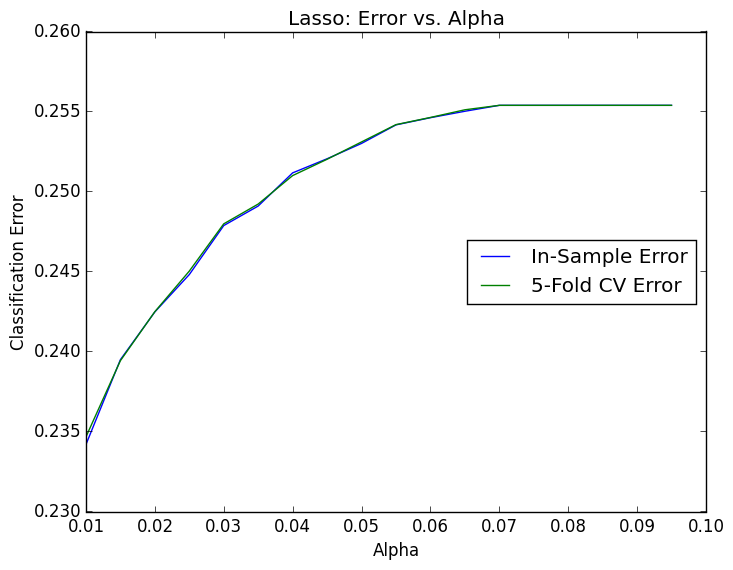
\includegraphics[scale=0.35]{lasso-vs-alpha2}
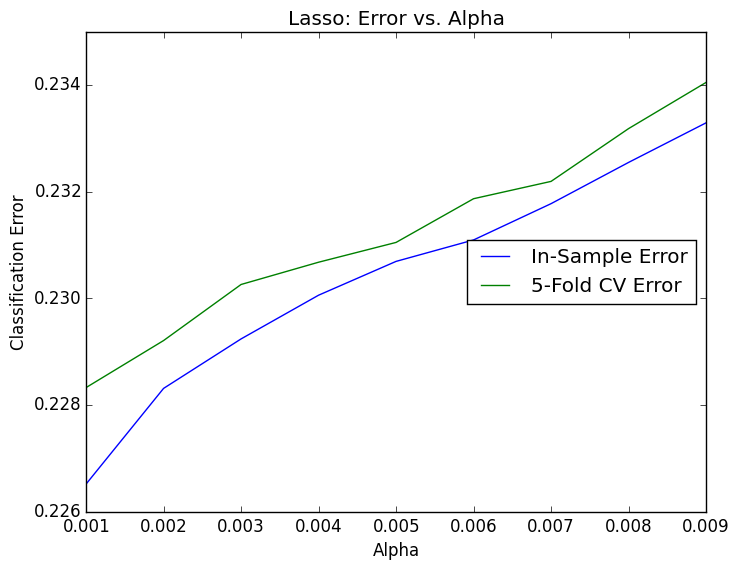
\includegraphics[scale=0.35]{lasso-vs-alpha}
\caption{Lasso Regression vs. Alpha. The effect of the regularization term alpha appears to negatively effect both in-sample and validation error, demonstrating underfitting.}
\end{figure}
In ridge regression, we found a regularization alpha that best minimized the validation at around alpha 20. This alpha appeared to reduce some level of overfitting because from alpha 0 to 20, in-sample error increased  while validation error decreased, although slightly.
\begin{figure}[H]
\centering
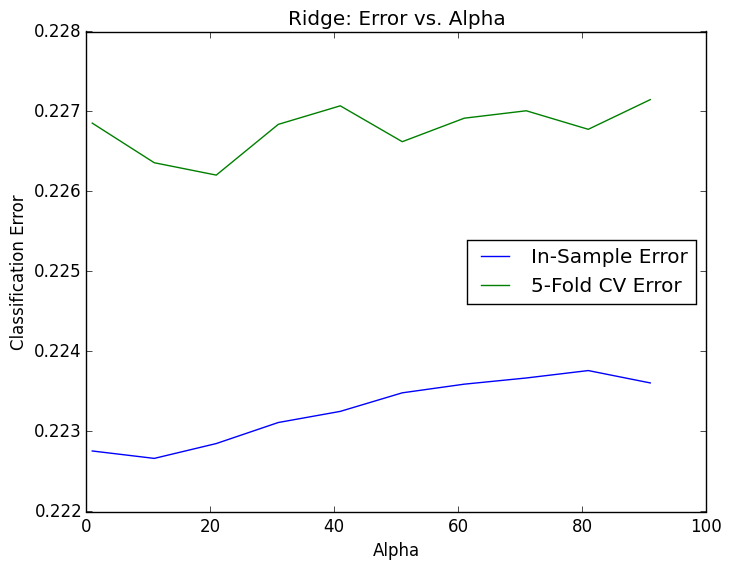
\includegraphics[scale=0.25]{ridge-vs-alpha}
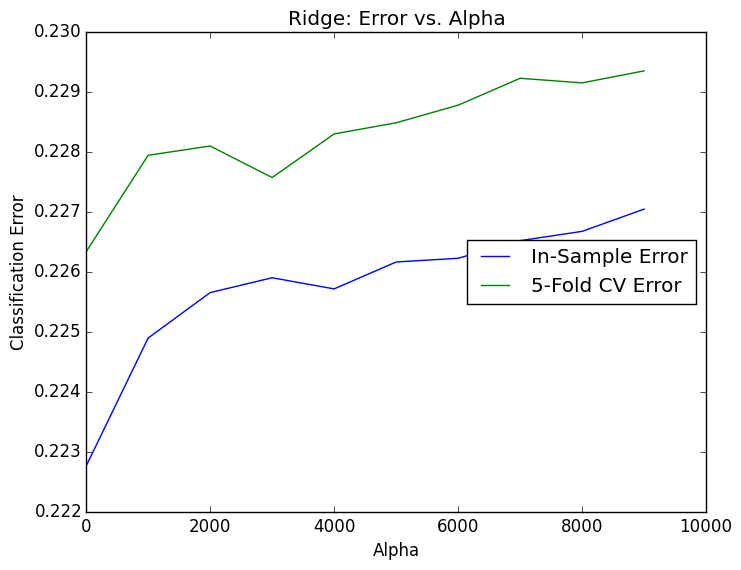
\includegraphics[scale=0.25]{ridge-vs-alpha3}
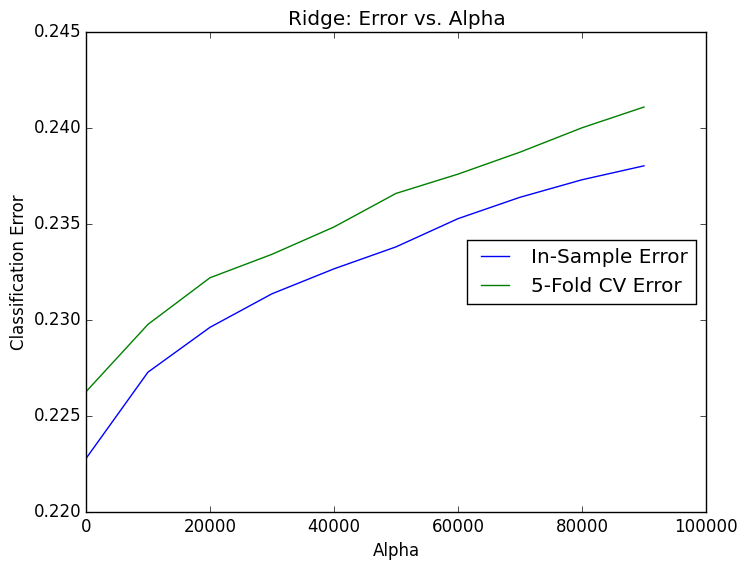
\includegraphics[scale=0.25]{ridge-vs-alpha2}
\caption{Ridge Regression vs. Alpha. The effect of the regularization appears to benefit the model when it is at a small value of $\alpha=20$.}
\end{figure}
In stochastic gradient descent, regularization proved to benefit the model as well, as shown in the plots below.
\begin{figure}[H]
\centering
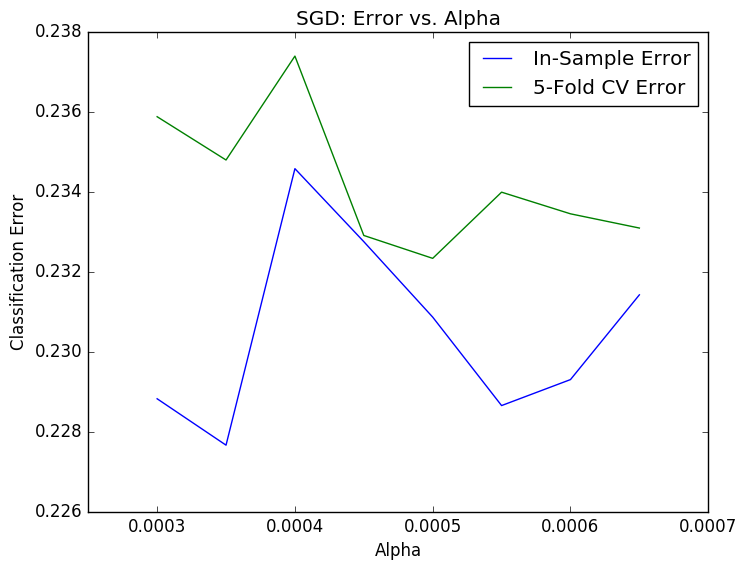
\includegraphics[scale=0.35]{sgd-vs-alpha}
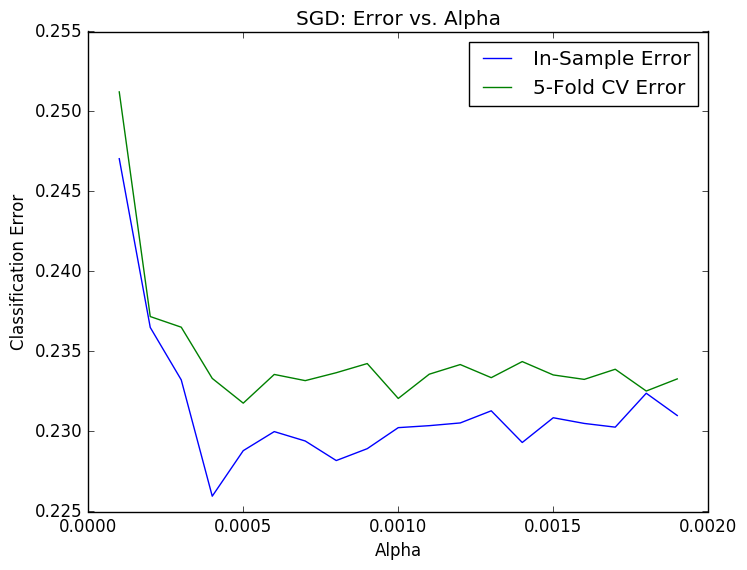
\includegraphics[scale=0.35]{sgd-vs-alpha2}
\caption{SGD vs. Alpha. Regularization appeared to reduce overfitting until alpha was 0.0005.}
\end{figure}
Finally, in SGD, we measured the effect of the number of epochs. By manually capping the number of epochs, we aimed to implement early-stopping and prevent over fitting. We did not find statistically conclusive evidence for overfitting, since the errors ranged within 0.005 as the number of epochs changed. However, we can see under-fitting under 500 iterations as both training and validation error fell as the number of iterations was increased. Although not conclusive due to dip in in-sample error too, the validation error dipped at 2500 epochs, suggesting a benefit to early stopping.
\begin{figure}[H]
\centering
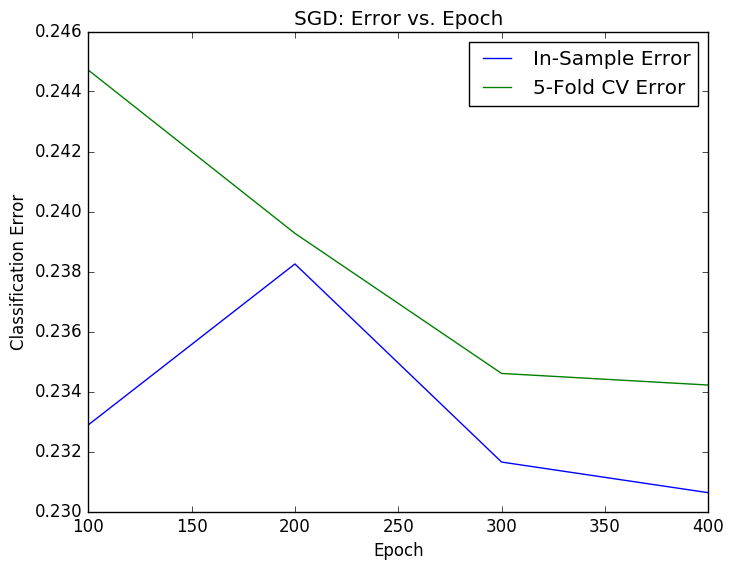
\includegraphics[scale=0.25]{sgd-vs-epoch2}
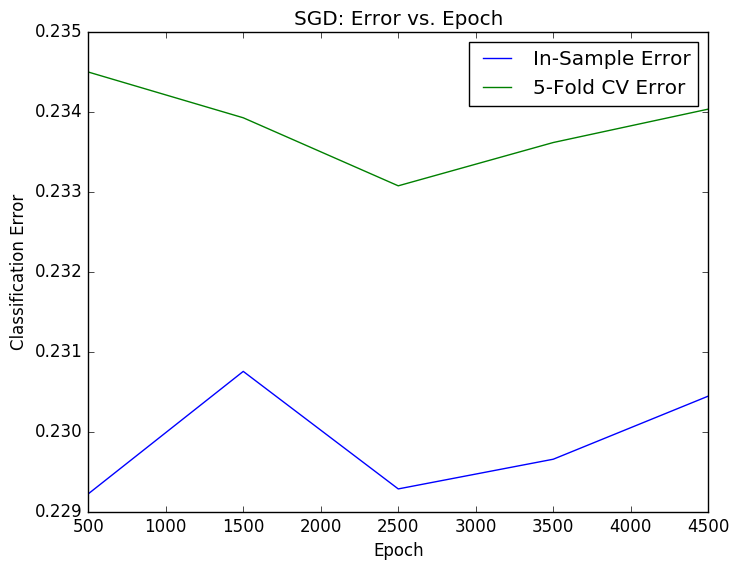
\includegraphics[scale=0.25]{sgd-vs-epoch3}
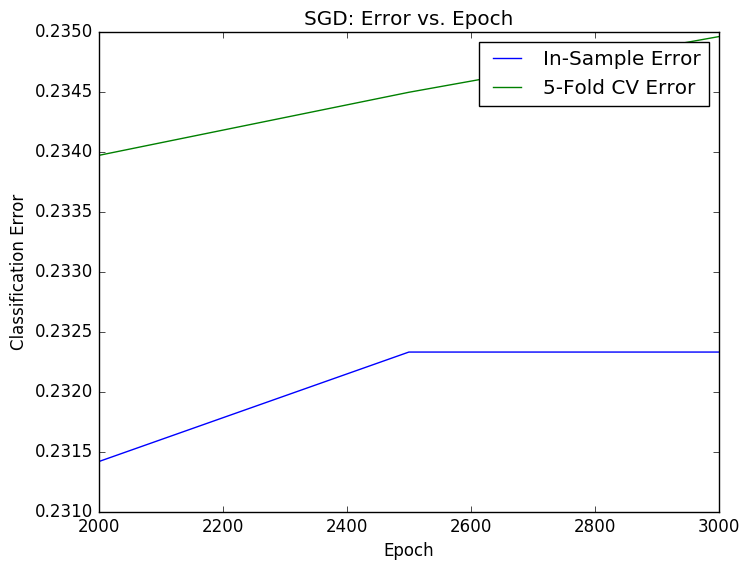
\includegraphics[scale=0.25]{sgd-vs-epoch4}
\caption{SGD vs. Epoch. We were able to determine that at least 500 iterations were needed to significantly fit the data without increasing validation error.}
\end{figure}
With other linear models, such as linear regression and SVM, there were less parameters to adjust and the computation took longer. However, similar analysis was done by measuring the differences in cross validations with different parameters, as seen in Table 1 (see Appendix).
\end{itemize}

\end{itemize}



\section{Model Selection}
\medskip
\begin{itemize}

    \item \boldline{Scoring} \\
    Due to the binary output classification, we chose to do scoring by classification accuracy (as opposed to loss measure). As shown in the cross validation results in Table 1, amongst the linear classifiers, Logistic Regression performed best on the pre-processed categorized data, although all had very similar results, except SVM, which performed significantly worse. Additionally, the neural network (MLP Classifier), even after efforts to optimize its parameters, could not perform near the level of the linear regressors. After the de-categorization of the data into around 5000 labels, many of the linear regressors performed worse, whereas the SVM and the stochastic gradient descent that performed worse before, performed better. However, the conversion of the data into labels with real-valued meaning significantly benefited the training of the neural networks, which we surmise is due to the fact that the categorical labels posses greater correlation to the output when considered together, which are the types of patterns that the neural network naturally performs better with.

    \item \boldline{Validation and Test} \\
    We used 5-fold cross-validation for all model selection and choosing semi-finalists of the neural-network models, except for choosing the finalists in the neural network models, where we used 10-fold cross-validation.  By generating these cross validations, we were able to select the optimal learning parameters, such as regularization terms, early stopping (max iterations), and loss functions. This was done by manually fixing all parameters except for one, optimizing that parameter, then moving on to optimizing another parameter, before circling back to the same parameter. In a way, we performed a manual step-wise gradient-like descent on parameters. The results of cross validation for various models can be seen in Table \# in the Appendix. The parameters variables refer to the API SKlearn's definition of parameters.

\end{itemize}



\section{Conclusion}
\medskip
\begin{itemize}

    \item \boldline{Discoveries} \\
    The main discovery from this competition was the difficulty of fitting a ``hard" and imbalanaced dataset, and in particular the challenges accompanying creating a model both sufficiently able to fit a training dataset (2008 data) and sufficiently general to adapt to an unknown and distinct new dataset (2012 data). These challenges will be analyzed in more depth in the section below.

    In terms of models used, we experimented with variants of common models examined in class. In particular, we utilized variations of trees aside from the default CART tree and various linear models. While our best performing models remained standard neural networks (and, on the test dataset, random forests), we certainly learned more about the variants of these models currently in use. In using neural networks, we discovered significant variation between different runs on the same model. In order to compensate for this, we utilized ensembles of networks, which we found improved on consistency and generalization ability.

    In examining the occasionally massive changes in the leaderboard between the first and second parts of the competition, and in examining the differing performances of our own models on these two datasets, we also discovered the dangers of overfitting and the propensities of various models for doing so. In particular, we found (after submission) that our more ``general" models (i.e., collections of networks and forests) tended to perform reasonably well on the new dataset, whereas models more prone to overfitting (smaller forests and networks, linear models) tended to suffer more. Considering the large drops experienced by many teams initially above us on the leaderboard, it is our belief that this ``overfitting the leaderboard" was in fact a fairly general problem.

    \item \boldline{Challenges} \\
    As mentioned above, the main problem experienced in the competition was the dataset. In particular, we found that the dataset was lopsided (~75\% of those polled voted), rather different from the test set (in which ~65\% of those polled voted), and very noisy (i.e., even the best/most overfitted models were unable to break 80\% classification accuracy). In dealing with such a dataset, we found that most models performed within a percent or two of each other, which made distinguishing the best models somewhat difficult. Further, it meant that it was very easy to fall into a trap of overfitting (i.e., gridsearching parameters, submitting an excessive number of models, and falsely concluding that the models that best fit the data did so because they were the best models). We managed to avoid this reasonably well, although we could have improved on our part 2 score had we selected better. Were we to do this competition again, we would have put more thought into how to best select models.

    Within the dataset, we also found that many of the parameters were either repeated, arbitrary (i.e., identification numbers), or answered for only a very small number of responders (i.e., several questions focused very specifically on certain subsets of the population, and therefore had response rates in the hundreds). We curated the dataset and removed many of these parameters from consideration, although determining whether or not a parameter should be included was not always a clear decision. Were we to redo this competition, we would have curated the dataset in a more principled (and, ideally, automated) manner, through some manner of cross-validation on model performance with various parameters removed. We would also likely have removed even more parameters; it is our belief that this might help with the generalization accuracy of the model.

    Another challenge we faced was with TensorFlow. We sunk a significant quantity of time in trying to get TensorFlow to train on the data, but ultimately it was unsuccessful. No matter what parameters we chose (network dimensions, initial weights, activation functions), the network trained in the exact same way, converging to 0.7446 in sample accuracy and predicting that all data points are voters. Even after we curated the data, TensorFlow still converged to this value. Ultimately, we resorted to using sklearn's implementation of a neural network and that ended up being our best performing model. \\

    We additionally encountered problems with resource limitations in training large models. While most of our models trained in reasonable time, we found that some (in particular, certain variants of random forests and SVMs) were slow enough to be infeasible, in addition to using massive amounts of memory ($> $ 10 GB). \\

\end{itemize}

\section{Appendix}

\def\arraystretch{1.1}%Line spacing in table, 1 is default
\begin{longtable}{c|c|c|c}
\caption{With data normalization, without de-categorization of data (does not include all tests)}\\\hline
Type & K-Folds & Parameters & Classification Accuracy \\\hline
SVM & 5 & 4-degree polynomial kernel & 0.7568 \\\hline
SVM & 5 & RBF kernel & 0.76797 \\\hline
Logistic Regression & 5 & \makecell*{SAG solver, 25 iterations (converged),\\ $10^{-5}$ regularization strength} & 0.774 \\\hline
Logistic Regression & 5 & \makecell*{SAG solver, 25 iterations (no \\convergence), $C=10^{0}$ regularization strength} & 0.773 \\\hline
Logistic Regression & 5 & \makecell*{SAG solver, 100 iterations (no \\convergence), $C=10^{0}$ regularization strength} & 0.773 \\\hline
Logistic Regression & 5 & \makecell*{SAG solver, 100 iterations (no \\convergence), $C=10^{5}$ regularization strength} & 0.773 \\\hline
Logistic Regression & 5 & \makecell*{SAG solver, 400 iterations (no \\convergence), $C=10^{0}$ regularization strength} & 0.773 \\\hline
Logistic Regression & 5 & \makecell*{Liblinear solver, 100 iterations (no \\convergence), $C=10^{0}$ regularization strength} & 0.774 \\\hline
Ridge Regression & 5 & \makecell*{$\alpha=20$ regularization strength,\\ (optimal alpha found by plotting CV vs. alpha)} & 0.7738 \\\hline
Lasso Regression & 5 & \makecell*{$\alpha=10^{-3}$ regularization strength,\\ (optimal alpha found by plotting CV vs. alpha)} & 0.7718 \\\hline
% Can explain why switched from early stopping tolerance to fixed max iterations
MLP$^{*}$ Classifier & 5 & \makecell*{Hidden layers=(200,100), iterations=5 \\ (optimal iterations found by plotting CV vs. iter.)} & 0.7711 \\\hline
MLP$^{*}$ Classifier & 5 & \makecell*{Hidden layers=(100), iterations=3 \\ (optimal iterations found by plotting CV vs. iter.)} & 0.7726 \\\hline
MLP$^{*}$ Classifier & 5 & \makecell*{Hidden layers=(100, 50, 10), iterations=4 \\ (optimal iterations found by plotting CV vs. iter.)} & 0.7725 \\\hline
MLP$^{*}$ Classifier & 5 & \makecell*{Hidden layers=(20), iterations=10 \\ (optimal iterations found by plotting CV vs. iter.)} & 0.7734 \\\hline
MLP$^{*}$ Classifier & 5 & \makecell*{Hidden layers=(20, 20), iterations=15 \\ (optimal iterations found by plotting CV vs. iter.)} & 0.7733 \\\hline
MLP$^{*}$ Classifier & 5 & \makecell*{Hidden layers=(20, 20,20), iterations=10 \\ (optimal iterations found by plotting CV vs. iter.)} & 0.7730 \\\hline
MLP$^{*}$ Classifier & 5 & \makecell*{Hidden layers=(200,100), iterations=5 \\ (optimal iterations found by plotting CV vs. iter.)} & 0.7711 \\\hline
\caption{Without data normalization, with de-categorization of data}\\\hline
SVM & 5 & RBF kernel & 0.7707 \\\hline
Logistic Regression & 5 & \makecell*{Liblinear solver, 50 iterations (converged) \\ $C=1$ regularization strength} & 0.7725 \\\hline
Logistic Regression & 5 & \makecell*{Liblinear solver, 100 iterations (converged)\\ $C=1$ regularization strength} & 0.7725 \\\hline
SGD & 5 & \makecell*{Hinge loss, 1000 iterations,\\ $\alpha=0.001$ regularization strength} & 0.7748 \\\hline
SGD & 5 & \makecell*{Hinge loss, 500 iterations,\\ $\alpha=0.001$ regularization strength} & 0.7737 \\\hline
SGD & 5 & \makecell*{Hinge loss, 100 iterations,\\ $\alpha=0.001$ regularization strength} & 0.7727 \\\hline
\caption{Finalists from 43 cross validations of various layer dimensions and iterations (bounded cross validation by iterations on both sides, such that an increase or decrease in iterations increased validation error significantly):}\\\hline
MLP$^{*}$ Classifier & 10 & \makecell*{Hidden layers=(50, 50), iterations=4 \\ (optimal iterations found by plotting CV vs. iter.)} & 0.7775 \\\hline
MLP$^{*}$ Classifier & 10 & \makecell*{Hidden layers=(100, 50, 10), iterations=9 \\ (optimal iterations found by plotting CV vs. iter.)} & 0.7782 \\\hline
MLP$^{*}$ Classifier & 10 & \makecell*{Hidden layers=(150, 50), iterations=5 \\ (optimal iterations found by plotting CV vs. iter.)} & 0.7776 \\\hline
MLP$^{*}$ Classifier & 10 & \makecell*{Hidden layers=(150, 50, 10), iterations=6 \\ (optimal iterations found by plotting CV vs. iter.)} & 0.7781 \\\hline

\caption{$^{*}$MLP = Multilayered Perceptron. $^{*}$SGD = Stochastic Gradient Descent. We saw de-categorization improve performance significantly in neural network models, whereas linear models performed slightly worse.}
\end{longtable}

\end{document}